\chapter{Specifikacija programske potpore}
		
	\section{Funkcionalni zahtjevi}
			
			
			\noindent \textbf{Dionici:}
			
			\begin{packed_enum}
				
				\item Dentalne klinike
				\item Vlasnici smještaja			
				\item Prijevoznici
				\item Administratori koji koriste aplikaciju
				\item Klijenti, tj. pacijenti
				\item Razvojni tim
				
				
			\end{packed_enum}
			
			\noindent \textbf{Aktori i njihovi funkcionalni zahtjevi:}
			
			
			\begin{packed_enum}
				\item  \underbar{Smještajni administrator (inicijator) može:}
				
				\begin{packed_enum}
					
					\item Pregledavati podatke o smještajima (tip, ocjena, adresa, period dostupnosti)
					\item Dodavati nove korisnike (ne klijente nego korisnike sustava)
					\item Korisnicima dodavati nove uloge
					\item Dodavati, izmjenjivati i brisati podatke o smještaju
					\item Vidjeti prikaz smještaja na karti
					
				\end{packed_enum}
				\eject
				
					\item  \underbar{Prijevoznički administrator (inicijator) može:}
				
				\begin{packed_enum}
					
					\item Pregledavati podatke o prijevoznicima
					\item Dodati osnovne osobne podatke prijevoznika
					\item Dodati kontaktne podatke i podatke o vrsti i kapacitetu vozila
					\item Izmjenjivati neosnovne podatke (kontakt, vrsta i kapacitet vozila)
					\item Izbrisati prijevoznika

				\end{packed_enum}
				
					\item  \underbar{Korisnički administrator (inicijator) može:}
				
				\begin{packed_enum}
					
					\item Dodati podatke o klijentima (osobni podatci, kontakt, preferencije o smještaju)
					
				\end{packed_enum}
			
				\item  \underbar{Baza podataka (sudionik) može:}
				
				\begin{packed_enum}
					
					\item Pohranjuje sve podatke o prijevoznicima
					\item Pohranjuje sve podatke o smještaju
					\item Pohranjuje nemedicinske podatke o klijentima
					
				\end{packed_enum}
				
					
			\end{packed_enum}
			
			\eject 
			

					
					\noindent \underbar{\textbf{UC1 - Prijava smještajnog administratora}}
					\begin{packed_item}
						
						\item \textbf{Glavni sudionik: }Smještajni administrator
						\item  \textbf{Cilj:} Prijaviti se u sustav kao smještajni administrator
						\item  \textbf{Sudionici:} Baza podataka
						\item  \textbf{Opis osnovnog tijeka:}
						
						\item[] \begin{packed_enum}
							
							\item Unos korisničkog imena i lozinke te odabir uloge smještajnog administratora
							\item Potvrda o postojanju računa i ispravnosti podataka
							\item Pristup funkcijama smještajnog administratora
						\end{packed_enum}
						
						\item  \textbf{Opis mogućih odstupanja:}
						
						\item[] \begin{packed_item}
							
							\item[2.a] Uneseni podatci nisu u točnom formatu
							\item[] \begin{packed_enum}
								
								\item Obavijestiti korisnika koji podatci nisu u točnom formatu
								\item Korisnik mijenja potrebne podatke i pokušava opet
								
							\end{packed_enum}
							\item[2.b] Korisnički račun ne postoji, lozinka nije točna ili korisničko ime nije točno
							\item[] \begin{packed_enum}
								
								\item Obavijestiti korisnika da su korisničko ime ili lozinka netočni
								\item Korisnik mijenja potrebne podatke i pokušava opet
								
							\end{packed_enum}

							
						\end{packed_item}
					\end{packed_item}
				
				\noindent \underbar{\textbf{UC2 - Prijava prijevoznog administratora}}
				\begin{packed_item}
					
					\item \textbf{Glavni sudionik: }Prijevozni administrator
					\item  \textbf{Cilj:} Prijaviti se u sustav kao prijevozni administrator
					\item  \textbf{Sudionici:} Baza podataka
					\item  \textbf{Opis osnovnog tijeka:}
					
					\item[] \begin{packed_enum}
						
						\item Unos korisničkog imena i lozinke te odabir uloge prijevoznog administratora
						\item Potvrda o postojanju računa i ispravnosti podataka
						\item Pristup funkcijama prijevoznog administratora
					\end{packed_enum}
					
					\item  \textbf{Opis mogućih odstupanja:}
					
					\item[] \begin{packed_item}
						
						\item[2.a] Uneseni podatci nisu u točnom formatu
						\item[] \begin{packed_enum}
							
							\item Obavijestiti korisnika koji podatci nisu u točnom formatu
							\item Korisnik mijenja potrebne podatke i pokušava opet
							
						\end{packed_enum}
						\item[2.b] Korisnički račun ne postoji, lozinka nije točna ili korisničko ime nije točno
						\item[] \begin{packed_enum}
							
							\item Obavijestiti korisnika da su korisničko ime ili lozinka netočni
							\item Korisnik mijenja potrebne podatke i pokušava opet
							
						\end{packed_enum}
						
						
					\end{packed_item}
				\end{packed_item}
				
				\noindent \underbar{\textbf{UC3 - Prijava korisničkog administratora}}
				\begin{packed_item}
					
					\item \textbf{Glavni sudionik: }Korisnički administrator
					\item  \textbf{Cilj:} Prijaviti se u sustav kao korisnički administrator
					\item  \textbf{Sudionici:} Baza podataka
					\item  \textbf{Opis osnovnog tijeka:}
					
					\item[] \begin{packed_enum}
						
						\item Unos korisničkog imena i lozinke te odabir uloge korisničkog administratora
						\item Potvrda o postojanju računa i ispravnosti podataka
						\item Pristup funkcijama korisničkog administratora
					\end{packed_enum}
					
					\item  \textbf{Opis mogućih odstupanja:}
					
					\item[] \begin{packed_item}
						
						\item[2.a] Uneseni podatci nisu u točnom formatu
						\item[] \begin{packed_enum}
							
							\item Obavijestiti korisnika koji podatci nisu u točnom formatu
							\item Korisnik mijenja potrebne podatke i pokušava opet
							
						\end{packed_enum}
						\item[2.b] Korisnički račun ne postoji, lozinka nije točna ili korisničko ime nije točno
						\item[] \begin{packed_enum}
							
							\item Obavijestiti korisnika da su korisničko ime ili lozinka netočni
							\item Korisnik mijenja potrebne podatke i pokušava opet
							
						\end{packed_enum}
						
						
					\end{packed_item}
				\end{packed_item}
				
				\noindent \underbar{\textbf{UC4 - Dodavanje novog korisnika}}
				\begin{packed_item}
					
					\item \textbf{Glavni sudionik: }Smještajni administrator
					\item  \textbf{Cilj:} Dodati novog korisnika sustava
					\item  \textbf{Sudionici:} Baza podataka
					\item  \textbf{Preduvjet:} Prijava smještajnog administratora
					\item  \textbf{Opis osnovnog tijeka:}
					
					\item[] \begin{packed_enum}
						
						\item Unos korisničkog imena i lozinke novog korisnika te odabir svih uloga koje će korisnik imati
						\item Provjera postoji li već korisnik s takvim imenom
						\item Upis novog korisnika u bazu podataka
					\end{packed_enum}
					
					\item  \textbf{Opis mogućih odstupanja:}
					
					\item[] \begin{packed_item}
						
						\item[2.a] Polja korisničko ime i/ili lozinka su prazni
						\item[] \begin{packed_enum}
							
							\item Obavijestiti korisnika koji su podatci prazni
							\item Korisnik mijenja potrebne podatke i pokušava opet
							
						\end{packed_enum}
						\item[2.b] Postoji korisnički račun s tim imenom
						\item[] \begin{packed_enum}
							
							\item Obavijestiti korisnika da postoji račun s tim imenom
							\item Korisnik mijenja korisničko ime i pokušava opet
							
						\end{packed_enum}
						\item[2.c] Nije odabrana niti jedna uloga
						\item[] \begin{packed_enum}
							
							\item Obavijestiti korisnika da račun mora imati neku ulogu
							\item Korisnik dodaje jednu ili više uloga i pokušava opet
							
						\end{packed_enum}
						
					\end{packed_item}
				\end{packed_item}
				
				\noindent \underbar{\textbf{UC5 - Pregled postojećih smještaja}}
				\begin{packed_item}
					
					\item \textbf{Glavni sudionik: }Smještajni administrator
					\item  \textbf{Cilj:} Pregledati postojeće smještaje
					\item  \textbf{Sudionici:} Baza podataka
					\item  \textbf{Preduvjet:} Prijava smještajnog administratora
					\item  \textbf{Opis osnovnog tijeka:}
					
					\item[] \begin{packed_enum}
						
						\item Smještajni administrator odabire opcije "Postojeći smještaji"
						\item Aplikacija u obliku liste prikazuje sve postojeće smještaje i kartu s njihovim adresama
					\end{packed_enum}

				\end{packed_item}
				
				\noindent \underbar{\textbf{UC6 - Dodavanje novog smještaja}}
				\begin{packed_item}
					
					\item \textbf{Glavni sudionik: }Smještajni administrator
					\item  \textbf{Cilj:} Dodati novi smještaj
					\item  \textbf{Sudionici:} Baza podataka
					\item  \textbf{Preduvjet:} Prijava smještajnog administratora
					\item  \textbf{Opis osnovnog tijeka:}
					
					\item[] \begin{packed_enum}
						
						\item Unos potrebnih podataka za dodavanje novog smještaja
						\item Provjera jesu li uneseni svi podatci
						\item Upis novog smještaja u bazu podataka
					\end{packed_enum}
					
					\item  \textbf{Opis mogućih odstupanja:}
					
					\item[] \begin{packed_item}
						
						\item[2.a] Neki od podataka nije unesen
						\item[] \begin{packed_enum}
							
							\item Obavijestiti korisnika koji podatci su prazni
							\item Korisnik mijenja potrebne podatke i pokušava opet
							
						\end{packed_enum}
						
					\end{packed_item}
				\end{packed_item}
				
				\noindent \underbar{\textbf{UC7 - Promjena podataka smještaja}}
				\begin{packed_item}
					
					\item \textbf{Glavni sudionik: }Smještajni administrator
					\item  \textbf{Cilj:} Promijeniti podatke smještaja
					\item  \textbf{Sudionici:} Baza podataka
					\item  \textbf{Preduvjet:} Prijava smještajnog administratora
					\item  \textbf{Opis osnovnog tijeka:}
					
					\item[] \begin{packed_enum}
						
						\item Smještajni administrator odabire "Promijeni" opciju na smještaju
						\item Smještajni administrator mijenja podatke o smještaju
						\item Smještajni administrator sprema promjene
						\item Pregledava se ispravnost podataka
						\item Mijenjaju se podatci u bazi podataka
					\end{packed_enum}
					
					\item  \textbf{Opis mogućih odstupanja:}
					
					\item[] \begin{packed_item}
						
						\item[3.a] Smještajni administrator izlazi bez spremanja
						\item[] \begin{packed_enum}
							
							\item Podatci se ne spremaju u bazu podataka
							
						\end{packed_enum}
						
						\item[4.a] Neki od podataka nije unesen
						\item[] \begin{packed_enum}
							
							\item Obavijestiti smještajnog administratora koji podatci su prazni
							\item Smještajni administrator mijenja potrebne podatke i pokušava opet
							
						\end{packed_enum}
						
					\end{packed_item}
				\end{packed_item}
				
				\noindent \underbar{\textbf{UC8 - Brisanje smještaja}}
				\begin{packed_item}
					
					\item \textbf{Glavni sudionik: }Smještajni administrator
					\item  \textbf{Cilj:} Promijeniti podatke smještaja
					\item  \textbf{Sudionici:} Baza podataka
					\item  \textbf{Preduvjet:} Prijava smještajnog administratora
					\item  \textbf{Opis osnovnog tijeka:}
					
					\item[] \begin{packed_enum}
						
						\item Smještajni administrator odabire "Izbriši" opciju na smještaju
						\item Aplikacija šalje "jeste li sigurni?" upit smještajnom administratoru
						\item Ako je, smještaj se briše iz baze, u protivnom se ne desi ništa
					\end{packed_enum}

				\end{packed_item}
				
			\noindent \underbar{\textbf{UC9 - Pregled postojećih prijevoznika}}
			\begin{packed_item}
				
				\item \textbf{Glavni sudionik: }Prijevozni administrator
				\item  \textbf{Cilj:} Pregledati postojeće prijevoznike
				\item  \textbf{Sudionici:} Baza podataka
				\item  \textbf{Preduvjet:} Prijava prijevoznog administratora
				\item  \textbf{Opis osnovnog tijeka:}
				
				\item[] \begin{packed_enum}
					
					\item Prijevozni administrator odabire opcije "Postojeći prijevoznici"
					\item Aplikacija u obliku liste prikazuje sve postojeće prijevoznike
				\end{packed_enum}
				
			\end{packed_item}
			
			\noindent \underbar{\textbf{UC10 - Dodavanje novog prijevoznika}}
			\begin{packed_item}
				
				\item \textbf{Glavni sudionik: }Prijevozni administrator
				\item  \textbf{Cilj:} Dodati novog prijevoznika
				\item  \textbf{Sudionici:} Baza podataka
				\item  \textbf{Preduvjet:} Prijava prijevoznog administratora
				\item  \textbf{Opis osnovnog tijeka:}
				
				\item[] \begin{packed_enum}
					
					\item Unos potrebnih podataka za dodavanje novog prijevoznika
					\item Provjera jesu li uneseni svi podatci
					\item Upis novog prijevoznika u bazu podataka
				\end{packed_enum}
				
				\item  \textbf{Opis mogućih odstupanja:}
				
				\item[] \begin{packed_item}
					
					\item[2.a] Neki od podataka nije unesen
					\item[] \begin{packed_enum}
						
						\item Obavijestiti prijevoznog administratora koji podatci su prazni
						\item Prijevozni administrator mijenja potrebne podatke i pokušava opet
						
					\end{packed_enum}
					
				\end{packed_item}
			\end{packed_item}
			
			\noindent \underbar{\textbf{UC11 - Promjena podataka o prijevozniku}}
			\begin{packed_item}
				
				\item \textbf{Glavni sudionik: }Prijevozni administrator
				\item  \textbf{Cilj:} Promijeniti podatke o prijevozniku
				\item  \textbf{Sudionici:} Baza podataka
				\item  \textbf{Preduvjet:} Prijava prijevoznog administratora
				\item  \textbf{Opis osnovnog tijeka:}
				
				\item[] \begin{packed_enum}
					
					\item Prijevozni administrator odabire "Promijeni" opciju na postojećem prijevozniku
					\item Prijevozni administrator mijenja podatke o prijevozniku
					\item Prijevozni administrator sprema promijene
					\item Pregledava se ispravnost podataka
					\item Mijenjaju se podatci u bazi podataka
				\end{packed_enum}
				
				\item  \textbf{Opis mogućih odstupanja:}
				
				\item[] \begin{packed_item}
					
					\item[3.a] Prijevozni administrator izlazi bez spremanja
					\item[] \begin{packed_enum}
						
						\item Podatci se ne spremaju u bazu podataka
						
					\end{packed_enum}
					
					\item[4.a] Neki od podataka nije unesen
					\item[] \begin{packed_enum}
						
						\item Obavijestiti prijevoznog administratora koji podatci su prazni
						\item Prijevozni administrator mijenja potrebne podatke i pokušava opet
						
					\end{packed_enum}
					
				\end{packed_item}
			\end{packed_item}
			
			\noindent \underbar{\textbf{UC12 - Brisanje prijevoznika}}
			\begin{packed_item}
				
				\item \textbf{Glavni sudionik: }Prijevozni administrator
				\item  \textbf{Cilj:} Promijeniti podatke smještaja
				\item  \textbf{Sudionici:} Baza podataka
				\item  \textbf{Preduvjet:} Prijava prijevoznog administratora
				\item  \textbf{Opis osnovnog tijeka:}
				
				\item[] \begin{packed_enum}
					
					\item Prijevozni administrator odabire "Izbriši" opciju na prijevozniku
					\item Aplikacija šalje "jeste li sigurni?" upit prijevoznom administratoru
					\item Ako je, prijevoznik se briše iz baze, u protivnom se ne desi ništa
				\end{packed_enum}
				
			\end{packed_item}
			\eject
			\noindent \underbar{\textbf{UC13 - Dodavanje novog klijenta}}
			\begin{packed_item}
				
				\item \textbf{Glavni sudionik: }Korisnički administrator
				\item  \textbf{Cilj:} Dodati novog korisnika
				\item  \textbf{Sudionici:} Baza podataka
				\item  \textbf{Preduvjet:} Prijava korisničkog administratora
				\item  \textbf{Opis osnovnog tijeka:}
				
				\item[] \begin{packed_enum}
					
					\item Unos potrebnih podataka za dodavanje novog korisnika
					\item Dohvat medicinskih podataka o korisniku
					\item Provjera jesu li uneseni svi podatci
					\item Dodjela smještaja klijentu
					\item Slanje poruke elektroničke pošte klijentu i prijevozniku o zaključenom planu 

				\end{packed_enum}
				
				\item  \textbf{Opis mogućih odstupanja:}
				
				\item[] \begin{packed_item}
					
					\item[2.b] Ne mogu se dohvatiti medicinski podatci
					\item[] \begin{packed_enum}
						
						\item Aplikacija ponovno pokušava dohvatiti podatke
						\item Ako je podatke nemoguće dohvatiti, nemoguće je unijeti novog korisnika
						
					\end{packed_enum}
					
					\item[3.a] Neki od podataka nije unesen
					\item[] \begin{packed_enum}
						
						\item Obavijestiti korisničkog administratora koji podatci su prazni
						\item Korisnički administrator mijenja potrebne podatke i pokušava opet
						
					\end{packed_enum}
					
				\end{packed_item}
			\end{packed_item}
			
				\eject
				\subsubsection{Dijagrami obrazaca uporabe}
					\eject
					\begin{figure}[htbp]
						\centering
						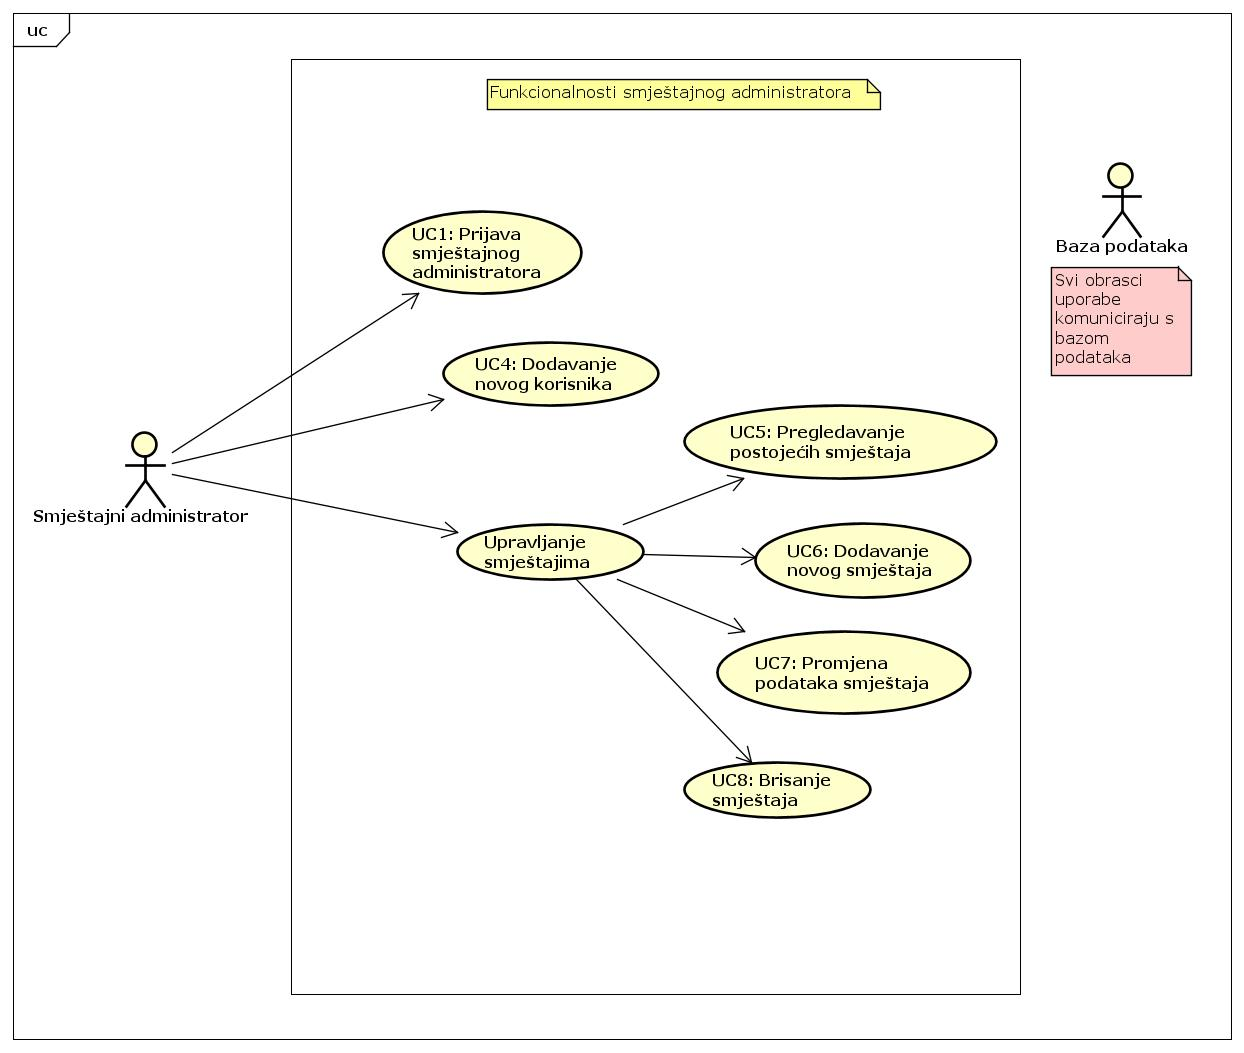
\includegraphics[width=0.9\textwidth]{dijagrami/fun_house}
						\caption{Funkcijski zahtjevi smještajnog administratora}
						\label{fig:funHouse}
					\end{figure}
					\begin{figure}[htbp]
						\centering
						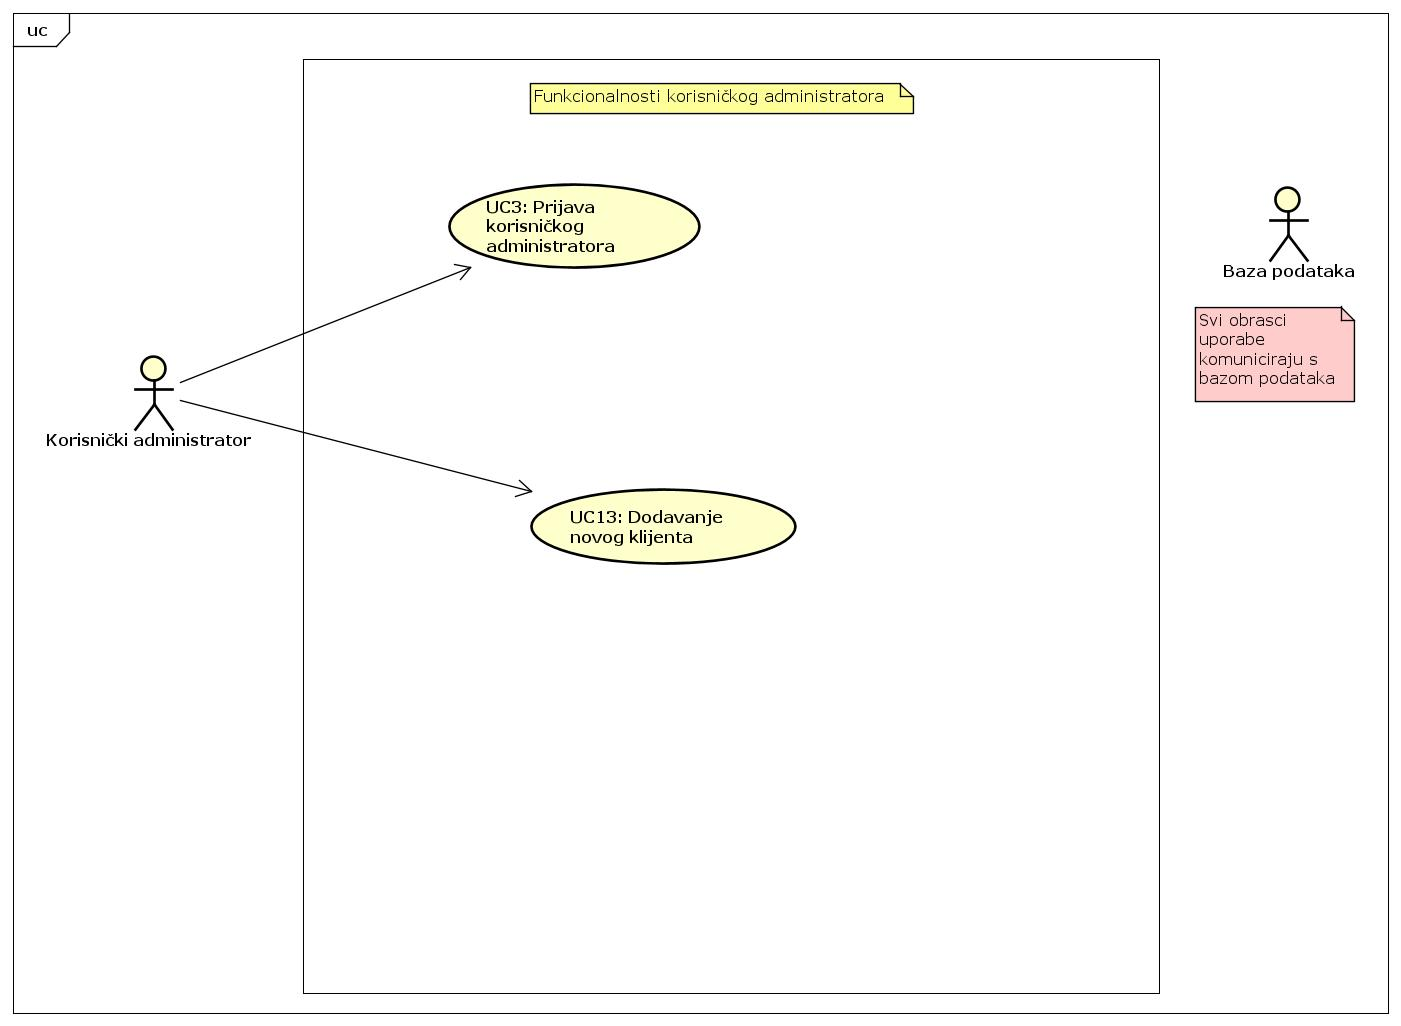
\includegraphics[width=0.9\textwidth]{dijagrami/fun_trans}
						\caption{Funkcijski zahtjevi transportnog administratora}
						\label{fig:funTrans}
					\end{figure}
					\begin{figure}[htbp]
						\centering
						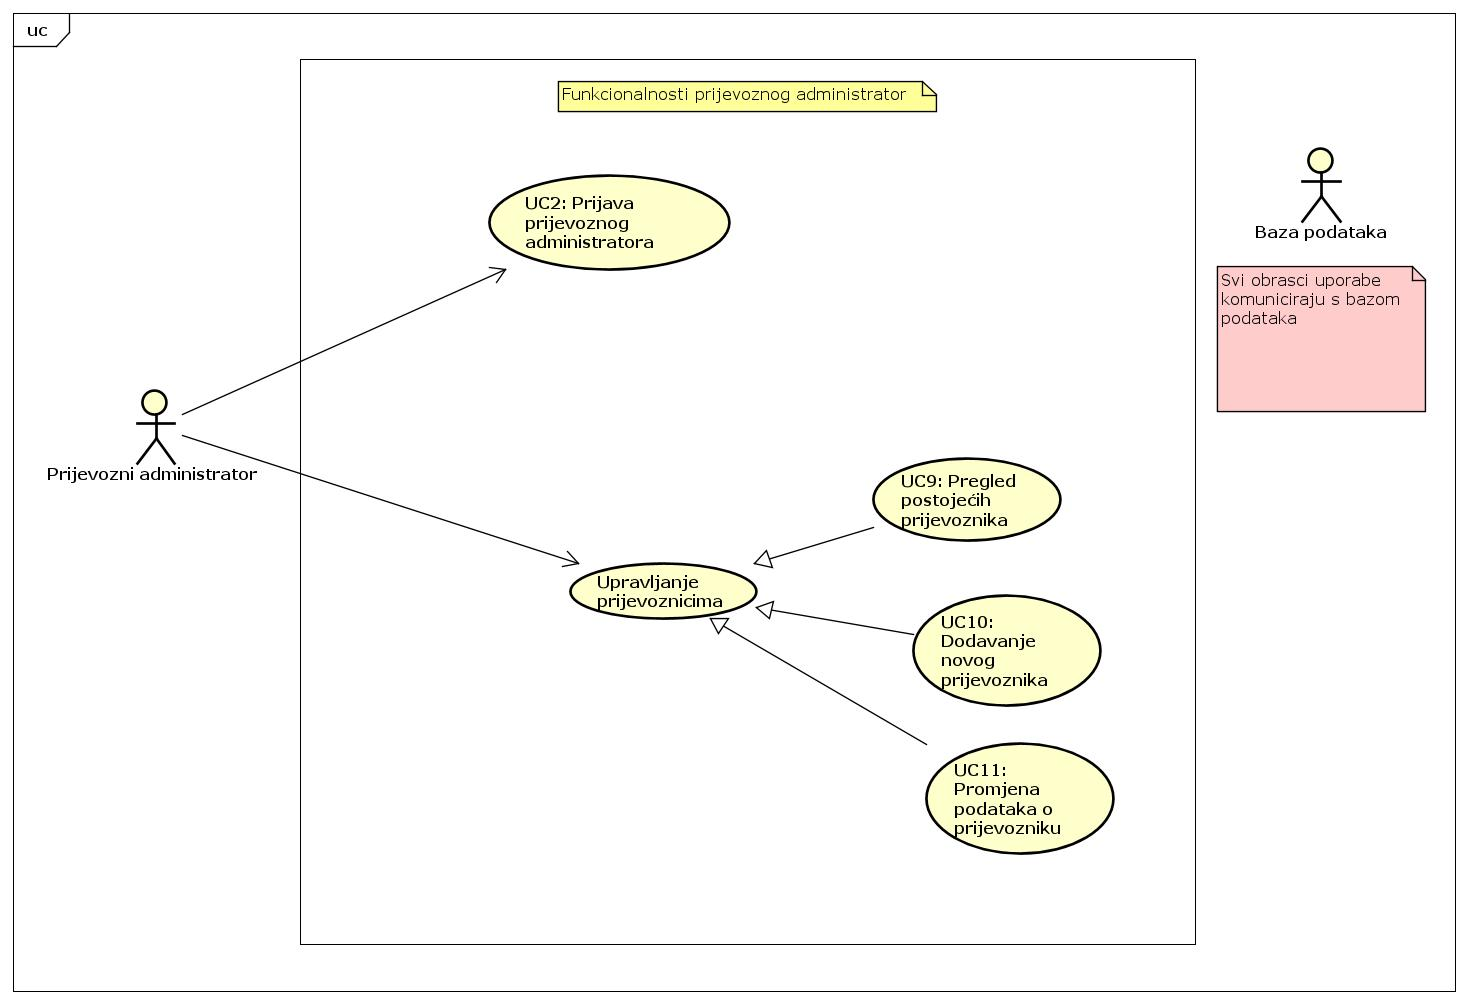
\includegraphics[width=0.9\textwidth]{dijagrami/fun_kor}
						\caption{Funkcijski zahtjevi korisničkog administratora}
						\label{fig:funKor}
					\end{figure}
				\eject		
				
			\subsection{Sekvencijski dijagrami}
			\textbf{Obrazac uporabe UC4: Dodavanje novog korisnika}
			
			Smještajni administrator odabire opciju dodaj novog korisnika. Web-aplikacija otvara obrazac za dodavanje novog korisnika. Smještajni administrator upisuje korisničko ime, lozinku i odabire uloge koje će novi administrator imati te šalje zahtjev aplikaciji. Aplikacija radi provjeru ispravnosti tih podataka i ako su ispravni šalje ih bazi podataka. Baza podataka provjerava postoji li već administrator s tim korisničkim imenom i ako ne postoji dodaje novog administratora. Smještajnom administratoru aplikacija javlja da je unos uspješno izvršen.
			\begin{figure}[htbp]
				\centering
				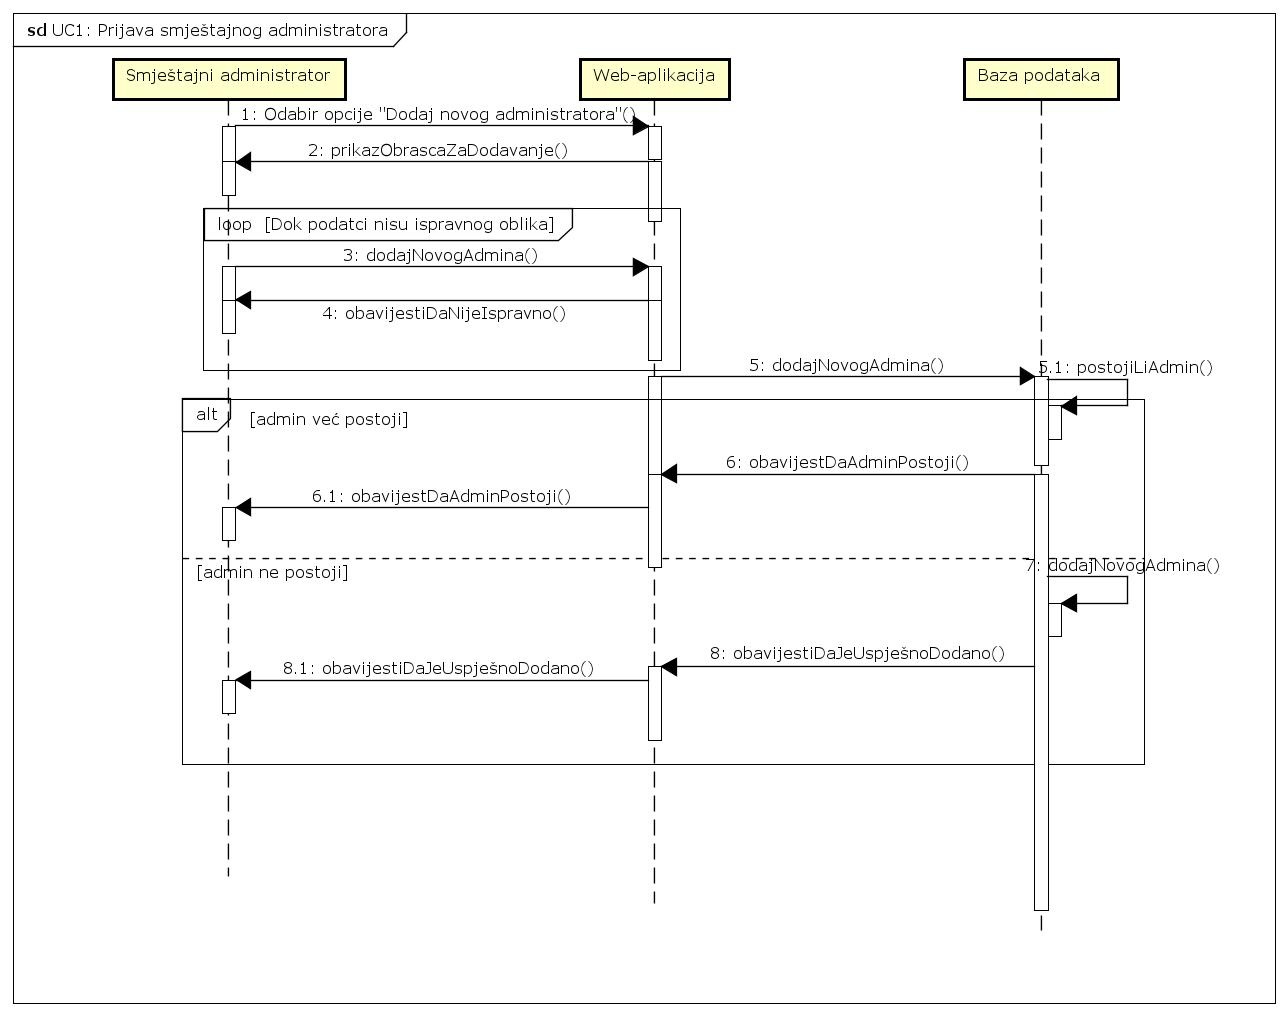
\includegraphics[width=0.9\textwidth]{dijagrami/sec_uc4}
				\caption{Sekvencijski dijagram za UC4}
				\label{fig:secUC4}
			\end{figure}
			\eject
			
			
			\textbf{Obrazac uporabe UC6: Dodavanje novog smještaja}
			
			Smještajni administrator odabire opciju dodaj novi smještaj. Web-aplikacija otvara obrazac za dodavanje novog smještaja. Smještajni administrator upisuje sve potrebne informacije za dodavanje smještaja. Ako su svi potrebni podatci ispunjeni aplikacija šalje podatke bazi podataka. Baza podataka registrira novi smještaj i vraća informaciju da je smještaj ispravno unesen.
			\begin{figure}[htbp]
				\centering
				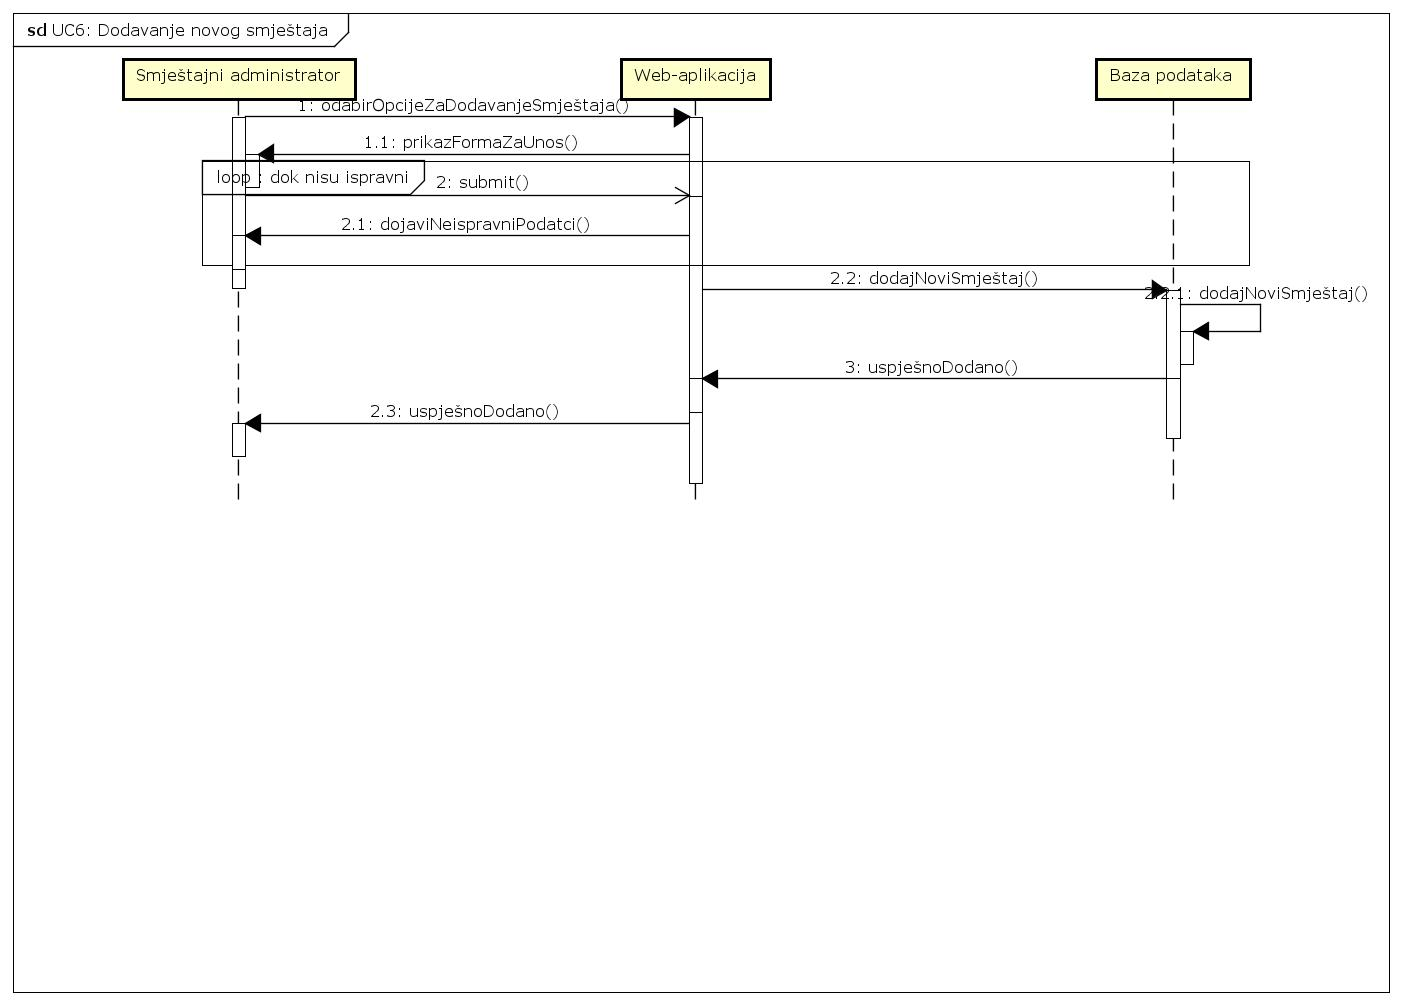
\includegraphics[width=0.9\textwidth]{dijagrami/sec_uc6}
				\caption{Sekvencijski dijagram za UC6}
				\label{fig:secUC6}
			\end{figure}
			\eject
			
						
			\textbf{Obrazac uporabe UC13: Dodavanje novog klijenta}
			
			Korisnički administrator odabire opciju dodaj novog korisnika. Aplikacija mu pokazuje obrazac za dodavanje novog klijenta. Nakon što upiše sve potrebne podatke aplikacija pokušava dohvatiti podatke od klijenta iz API-a klinike. Ako prvi put ne uspije pokušava opet, a ako i drugi put ne uspije javlja administratoru da trenutno unos nije moguć. Ako je dohvat uspješan klijent se dodaje u bazu podataka i aplikacija šalje poruku elektroničke pošte klijentu i prijevozniku odgovornom za klijenta, a administratoru se javlja da je unos uspješan.
			\begin{figure}[htbp]
				\centering
				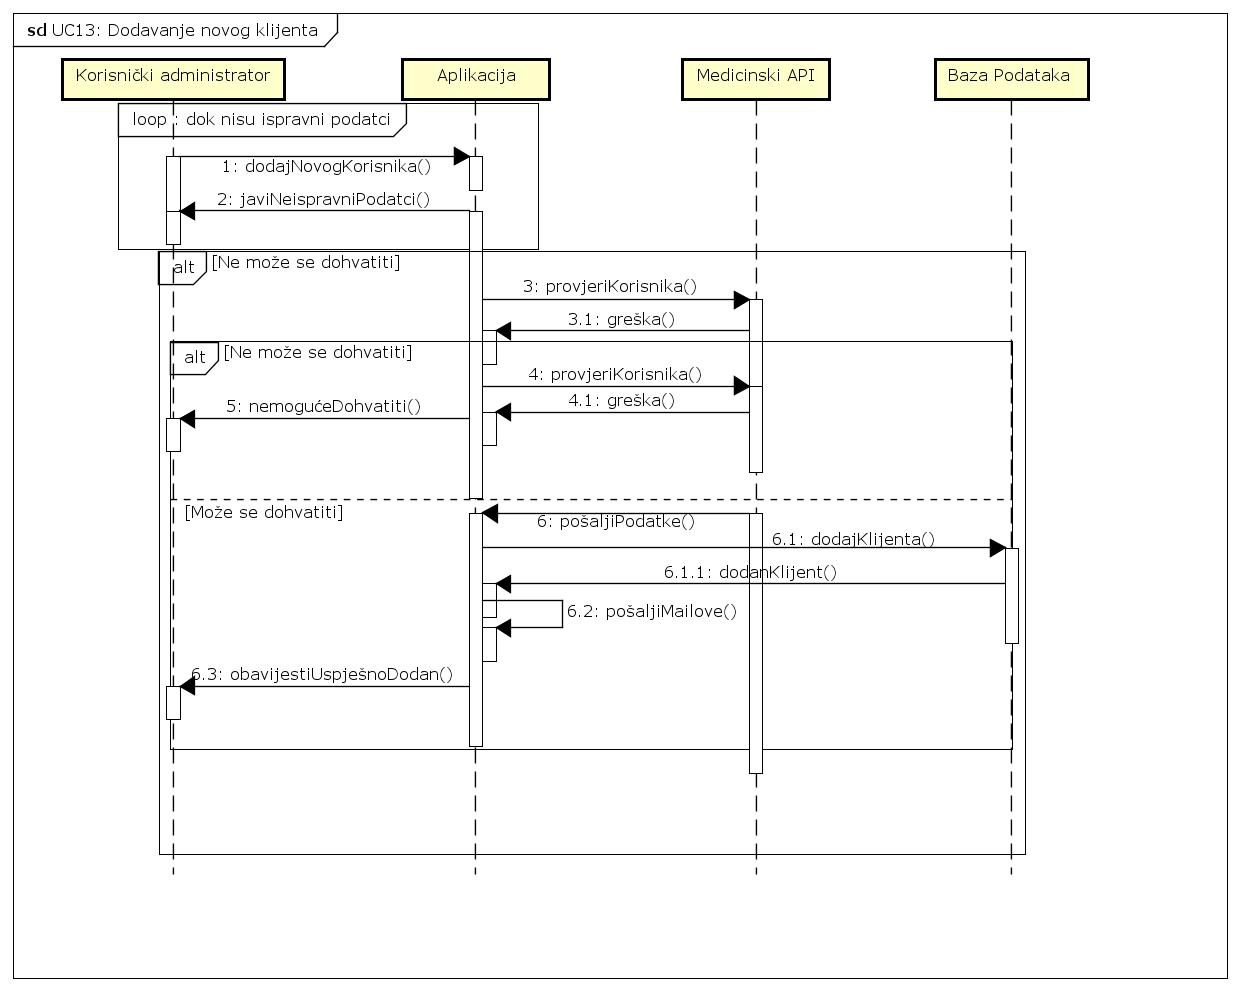
\includegraphics[width=0.9\textwidth]{dijagrami/sec_uc13}
				\caption{Sekvencijski dijagram za UC13}
				\label{fig:secUC13}
			\end{figure}
			\eject
			
				
	
		\section{Ostali zahtjevi}
		
		\begin{packed_item}
			\item Sustav treba omogućiti udaljeni pristup administratorima
			\item Sustav treba omogućiti istovremeni rad više korisnika
			\item Sve operacije s bazom podataka moraju biti sigurne, a lozinke zaštićene
			\item Sustav bilo kakve greške treba dojaviti administratorima na pregledan način umjesto da sruši sustav
			\item Sustav mora poslati pravilno formatirane poruke elektroničke pošte kako one ne bi završile u spam-u
			\item Sustav mora biti dovoljno općenito implementiran kako bi bio lagano nadogradiv
			\item Sustav mora biti izgrađen koristeći principe objektno orijentiranog programiranja
			\item Sustav mora biti jednostavno izgrađen i svi obavezni podatci za unos moraju biti jasno naznačeni
			\item Greška u unosu ne smije srušiti sustav
		\end{packed_item}
			 
			 
			 
	